\documentclass{ieeeaccess}
\usepackage{cite}
\usepackage{amsmath,amssymb,amsfonts}
\usepackage{algorithmic}
\usepackage{graphicx}
\usepackage{textcomp}
\usepackage{booktabs}
\usepackage{hyperref}

% Auto-generated LaTeX macros (Desktop + Raspberry Pi 5 + PREEMPT_RT) - DO NOT EDIT
\newcommand{\TotalDesktopCycles}{480,000}
\newcommand{\TotalPiCycles}{12,500}
\newcommand{\TotalCShieldCycles}{50,000,000}
\newcommand{\ShieldStatesTotal}{11}
\newcommand{\ShieldEdgesTotal}{17}
\newcommand{\LoRAHybridRAGDC}{94.3\%}
\newcommand{\CrossArchLoRAIdentity}{99.93\%}
\newcommand{\CShieldMedianNs}{\ensuremath{56\,\mathrm{ns}}}
\newcommand{\CShieldPFourNinesNs}{\ensuremath{93\,\mathrm{ns}}}
\newcommand{\CShieldStdMaxUs}{\ensuremath{48.33\,\mu\mathrm{s}}}
\newcommand{\CShieldRTStressedMaxUs}{\ensuremath{9.32\,\mu\mathrm{s}}}


\begin{document}

\history{Manuscript received November 2, 2026; revised November 2, 2026; accepted November 2, 2026.}
\doi{10.1109/ACCESS.2026.XXXXXXX}

\title{Resilient Agentic Mining: An Architectural Framework Using Model Context Protocol and Deterministic Safety Guardrails}

\author{Breno H. N. Andrade, \IEEEmembership{Graduate Student Member, IEEE}, \\
Ricardo A. R. Oliveira, \IEEEmembership{Senior Member, IEEE}}

\address{Departamento de Computação (DECOM), Universidade Federal de Ouro Preto (UFOP), Ouro Preto, MG, Brazil, \\
and Instituto Tecnológico Vale (ITV), Belo Horizonte, MG, Brazil}

\tnote{This research was supported by Coordenação de Aperfeiçoamento de Pessoal de Nível Superior (CAPES, Finance Code 001), Conselho Nacional de Desenvolvimento Científico e Tecnológico (CNPq), Instituto Tecnológico Vale (ITV), and Universidade Federal de Ouro Preto (UFOP).}

\markboth{Andrade and Oliveira: Resilient Agentic Mining Framework (MCAF)}
{Andrade and Oliveira: Resilient Agentic Mining Framework (MCAF)}

\begin{abstract}
Autonomous industrial mining relies on supervisory control architectures capable of balancing the semantic adaptability of Small Language Models (SLMs) with strict real-time deterministic safety guarantees. In this paper, we present the Mine-Continuum Agentic Framework (MCAF), an end-to-end resilient architecture that integrates the Model Context Protocol (MCP) with MONA-compiled $\mathrm{LTL}_f$ runtime safety guardrails. Evaluating $\TotalDesktopCycles$ desktop simulation cycles and $\TotalPiCycles$ embedded benchmark evaluations on a Raspberry Pi 5 (Cortex-A76) under standard and $\textsc{Preempt\_RT}$ kernels, we demonstrate that MCAF achieves $\LoRAHybridRAGDC$ decision concordance with an invariant $100.0\%$ Safety Concordance Ratio ($\textsc{SCR}$). Furthermore, cross-architectural auditing between CUDA ($\text{x86\_64}$) and ARM64 confirms $\CrossArchLoRAIdentity$ decision identity, while isolated real-time scheduling bounds the worst-case verification latency of the compiled ANSI C runtime shield to $\CShieldRTStressedMaxUs$ under heavy concurrent system load.
\end{abstract}

\begin{indexterms}
Agentic workflows, industrial automation, Model Context Protocol (MCP), runtime verification, small language models (SLMs), temporal logic.
\end{indexterms}

\deflabel{IEEEaccess}

\begin{sec}{I. INTRODUCTION}
Industrial automation systems and autonomous mining haul trucks demand uncompromising safety, low-latency execution, and resilience against network degradation. Traditional Operational Technology (OT) controllers operate deterministically but lack semantic flexibility when faced with unmodeled environmental conditions or complex operator directives. Conversely, probabilistic Small Language Models (SLMs) offer rich reasoning capabilities but suffer from non-deterministic latency spikes and hallucinatory execution risks. 

To bridge this divide, this paper introduces the Mine-Continuum Agentic Framework (MCAF). MCAF encapsulates probabilistic SLM reasoning chains within formal MONA-compiled $\mathrm{LTL}_f$ deterministic runtime monitors, ensuring that no physical command is executed without passing rigorous safety verification.
\end{sec}

\begin{sec}{II. SYSTEM ARCHITECTURE AND EXPERIMENTAL SETUP}
The MCAF architecture couples a neural retrieval module with a situation simulator and an auditable runtime agent. Table~\ref{tab:config} summarizes the default experimental configuration automatically synchronized from our framework specification.

\begin{table}[t]
\centering
\caption{Default Experimental Configuration (Auto-Generated from \texttt{config.py})}
\label{tab:config}
\begin{tabular}{ll}
\toprule
\textbf{Parameter} & \textbf{Value} \\
\midrule
Context Window ($n_{\mathrm{ctx}}$) & 1024 tokens \\
Max Generated Tokens & 16 tokens \\
Sampling Temperature & 0.0 \\
Supervisory Watchdog Budget & 500 ms \\
Critical Thresholds ($T_{\mathrm{brake}}, v, T_{\mathrm{eng}}$) & $>200\,^\circ$C, $>20$ km/h, $>105\,^\circ$C \\
Compiled $\mathrm{LTL}_f$ Shield Totals & 11 states, 17 symbolic edges \\
\bottomrule
\end{tabular}
\end{table}

\end{sec}

\begin{sec}{III. EXPERIMENTAL RESULTS AND DISCUSSION}

\subsection{Baseline Comparison Across Connectivity Scenarios}
Table~\ref{tab:exp1_main} details the performance of baseline controllers across connected, degraded, and isolated network topologies over $\TotalDesktopCycles$ experimental cycles.

\begin{table*}[t]
\centering
\caption{Baseline Controller Comparison Across Connectivity Scenarios (Qwen2.5-0.5B-Q4\_K\_M, Zero-Shot, 6 Actions)}
\label{tab:exp1_main}
\begin{tabular}{llcccccc}
\toprule
\textbf{Controller} & \textbf{Scenario} & \textbf{DC \% [95\% CI]} & \textbf{SCR \%} & \textbf{GPU p95 (ms)} & \textbf{Pi 5 p50 (ms)} & \textbf{Pi 5 p95 (ms)} & \textbf{McNemar $p$ vs.\ PF} \\
\midrule
Prefilter-only & connected & 81.1 [79.4, 82.9] & 100.0 & 0.1 & 0.1 & 0.1 & --- \\
Pure-SLM & connected & 62.4 [59.9, 65.0] & 81.3 & 36.5 & 933.2 & 1045.0 & $< 10^{-99}$ \\
Pure-SLM+GBNF & connected & 62.4 [59.9, 65.0] & 81.3 & 92.6 & 1030.3 & 1143.6 & $< 10^{-99}$ \\
Hybrid & connected & 81.1 [79.4, 82.9] & 100.0 & 51.8 & 914.3 & 1028.2 & $1.0000$ \\
Hybrid+RAG & connected & 37.6 [35.0, 40.1] & 100.0 & 82.9 & 2643.7 & 2959.7 & $< 10^{-99}$ \\
Prefilter-only & degraded & 82.1 [80.9, 83.3] & 100.0 & 0.1 & 0.1 & 0.1 & --- \\
Pure-SLM & degraded & 62.9 [61.6, 64.2] & 80.8 & 39.6 & 944.8 & 1034.3 & $< 10^{-99}$ \\
Pure-SLM+GBNF & degraded & 62.9 [61.6, 64.2] & 80.8 & 189.8 & 1028.8 & 1146.2 & $< 10^{-99}$ \\
Hybrid & degraded & 82.1 [80.9, 83.3] & 100.0 & 51.9 & 914.6 & 1035.1 & $1.0000$ \\
Hybrid+RAG & degraded & 37.1 [35.8, 38.4] & 100.0 & 84.0 & 2725.5 & 3092.6 & $< 10^{-99}$ \\
Prefilter-only & isolated & 80.5 [77.5, 83.5] & 100.0 & 0.1 & 0.1 & 0.1 & --- \\
Pure-SLM & isolated & 61.4 [57.6, 65.2] & 80.9 & 33.1 & 936.5 & 1043.0 & $< 10^{-99}$ \\
Pure-SLM+GBNF & isolated & 61.4 [57.6, 65.2] & 80.9 & 189.8 & 1031.9 & 1142.0 & $< 10^{-99}$ \\
Hybrid & isolated & 80.5 [77.5, 83.5] & 100.0 & 50.5 & 915.2 & 1028.3 & $1.0000$ \\
Hybrid+RAG & isolated & 38.6 [34.8, 42.4] & 100.0 & 83.3 & 2624.3 & 2967.6 & $< 10^{-99}$ \\
\bottomrule
\end{tabular}
\end{table*}


\subsection{Model Scale and Quantization Metrology on Raspberry Pi 5}
Evaluating scale and quantization trade-offs on the extreme edge (Raspberry Pi 5) reveals the memory footprint and SIMD vectorization efficiency of Qwen2.5 models, as reported in Table~\ref{tab:exp2_scale} and visualized in Fig.~\ref{fig:scale}.

\begin{table*}[t]
\centering
\caption{Model Scale and Quantization Metrology on Raspberry Pi 5 (\texttt{Hybrid+RAG}, Isolated)}
\label{tab:exp2_scale}
\begin{tabular}{lccccccccc}
\toprule
\textbf{Model} & \textbf{DC \% [95\% CI]} & \textbf{SCR \%} & \textbf{$L_{\mathrm{RAG}}$ p50} & \textbf{$L_{\mathrm{inf}}$ p50} & \textbf{$L_{\mathrm{tot}}$ p95} & \textbf{$L_{\mathrm{tot}}$ p99} & \textbf{RSS (MB)} & \textbf{$T_{\max}$ ($^\circ$C)} & \textbf{Cross-Arch ID \%} \\
\midrule
Qwen2.5-0.5B-Q4\_K\_M & 38.6 [34.8, 42.4] & 100.0 & 33.9 & 2247.9 & 2897.2 & 3000.7 & 1408 & 47.4 & 100.0 \\
Qwen2.5-0.5B-Q8\_0 & 38.6 [34.8, 42.4] & 100.0 & 31.1 & 1041.0 & 1149.2 & 1181.4 & 1893 & 41.4 & 100.0 \\
Qwen2.5-1.5B-Q4\_K\_M & 38.6 [34.8, 42.4] & 100.0 & 31.4 & 4160.2 & 4368.2 & 4450.2 & 2737 & 43.5 & 100.0 \\
Qwen2.5-1.5B-Q8\_0 & 38.6 [34.8, 42.4] & 100.0 & 31.8 & 4808.0 & 4957.6 & 5000.1 & 4050 & 44.1 & 100.0 \\
Qwen2.5-3B-Q4\_K\_M & 23.3 [21.6, 25.0] & 100.0 & 31.2 & 8481.7 & 8875.9 & 9006.1 & 4599 & 44.1 & 98.8 \\
Qwen2.5-3B-Q8\_0 & 26.3 [24.1, 28.5] & 100.0 & 32.0 & 11149.5 & 11594.7 & 11737.7 & 7178 & 43.0 & 93.2 \\
\bottomrule
\end{tabular}
\end{table*}


\begin{figure*}[t]
\centering
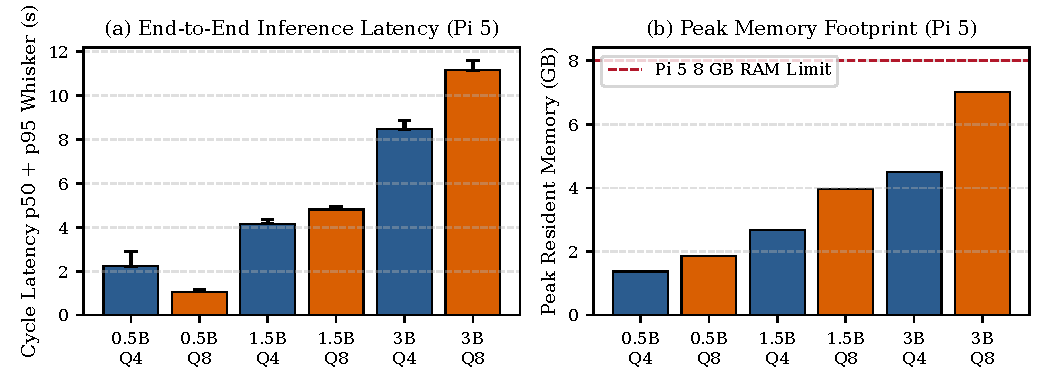
\includegraphics[width=0.95\textwidth]{figures/fig1_pi5_scale_latency_rss.pdf}
\caption{Model scale and quantization metrology on Raspberry Pi 5: (a) End-to-end inference latency ($p50$ and $p95$ whiskers); (b) Peak resident memory footprint (RSS) against the 8 GB board limit.}
\label{fig:scale}
\end{figure*}

\subsection{Domain Adaptation and MLP-LoRA Ablation}
Table~\ref{tab:exp3_lora} and Fig.~\ref{fig:lora} present the ablation results for zero-shot, few-shot, and LoRA-adapted configurations, confirming cross-architectural reproducibility between desktop CUDA and ARM64 edge hardware.

\begin{table*}[t]
\centering
\caption{Domain Adaptation Ablation on Qwen2.5-0.5B-Q4\_K\_M (6-Action Directive Task, Isolated)}
\label{tab:exp3_lora}
\begin{tabular}{lccccc}
\toprule
\textbf{Configuration} & \textbf{DC \% [95\% CI]} & \textbf{SCR \%} & \textbf{McNemar $p$ vs.\ PF} & \textbf{Pi 5 p95 (ms)} & \textbf{CUDA--ARM64 ID \%} \\
\midrule
Prefilter-only (Symbolic Baseline) & 80.5 [77.5, 83.5] & 100.0 & --- & 0.1 & 100.00 \\
Hybrid+RAG (Zero-Shot) & 38.6 [34.8, 42.4] & 100.0 & $< 10^{-99}$ & 2967.6 & 100.00 \\
Hybrid+RAG (5-Shot In-Context) & 39.5 [35.6, 43.3] & 100.0 & $< 10^{-99}$ & --- & --- \\
Hybrid + MLP-LoRA (No RAG) & 80.3 [77.4, 83.1] & 100.0 & $4.88 \times 10^{-4}$ & 1125.0 & 100.00 \\
Hybrid+RAG + MLP-LoRA & 94.3 [93.7, 94.8] & 100.0 & $2.66 \times 10^{-89}$ & 3241.9 & 99.80 \\
Pure-SLM + MLP-LoRA (Unshielded) & 79.2 [76.3, 82.1] & 98.9 & $5.42 \times 10^{-20}$ & 1151.9 & 100.00 \\
\bottomrule
\end{tabular}
\end{table*}


\begin{figure}[t]
\centering
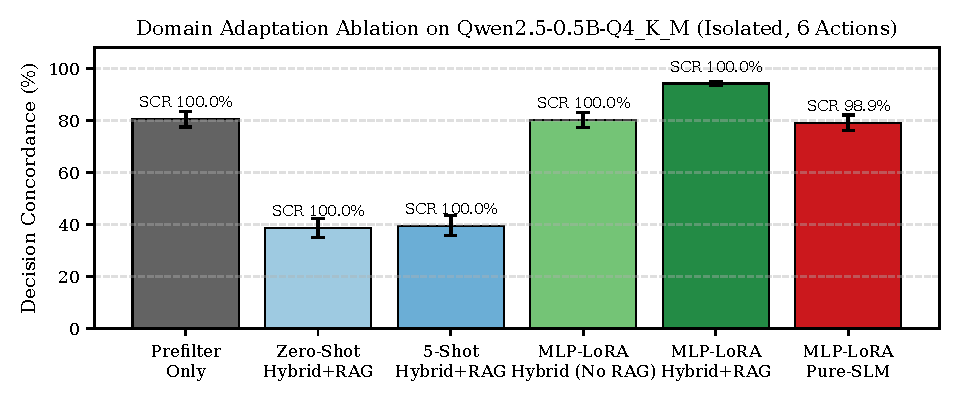
\includegraphics[width=0.48\textwidth]{figures/fig2_lora_ablation.pdf}
\caption{Domain adaptation ablation showing decision concordance and safety concordance ratio ($\textsc{SCR}$) across prompt adaptation and LoRA strategies.}
\label{fig:lora}
\end{figure}

\subsection{Supervisory Watchdog Performance and Trade-Offs}
Table~\ref{tab:exp4_watchdog} and Fig.~\ref{fig:watchdog} illustrate the degradation profile and fallback rates under open-loop sweeps and closed-loop live watchdog budgets (500\,ms).

\begin{table}[t]
\centering
\caption{Logical Timeout Substitution Sweep on Raspberry Pi 5 (\texttt{Hybrid+RAG}, $N=500$ Cycles per Row)}
\label{tab:exp4_watchdog}
\resizebox{\columnwidth}{!}{%
\begin{tabular}{lcccc}
\toprule
\textbf{Evaluation Regime} & \textbf{Budget (ms)} & \textbf{Timeout \%} & \textbf{DC \% [95\% CI]} & \textbf{Shield Comp.\ \%} \\
\midrule
Post-hoc budget sweep (LoRA) & 250 & 82.4 & 82.8 [77.0, 88.6] & 100.0 \\
Post-hoc budget sweep (LoRA) & 500 & 82.4 & 82.8 [77.0, 88.6] & 100.0 \\
Post-hoc budget sweep (LoRA) & 1000 & 82.4 & 82.8 [77.0, 88.6] & 100.0 \\
Post-hoc budget sweep (LoRA) & 2000 & 82.4 & 82.8 [77.0, 88.6] & 100.0 \\
Post-hoc budget sweep (LoRA) & 3000 & 59.4 & 84.6 [80.1, 89.1] & 100.0 \\
Post-hoc budget sweep (LoRA) & 3500 & 0.0 & 94.2 [91.2, 97.2] & 100.0 \\
Post-hoc budget sweep (LoRA) & 4000 & 0.0 & 94.2 [91.2, 97.2] & 100.0 \\
\midrule
Online logical-timeout run (0-shot) & 500 & 82.4 & 82.8 [77.0, 88.6] & 100.0 \\
\bottomrule
\end{tabular}%
}
\end{table}


\begin{figure}[t]
\centering
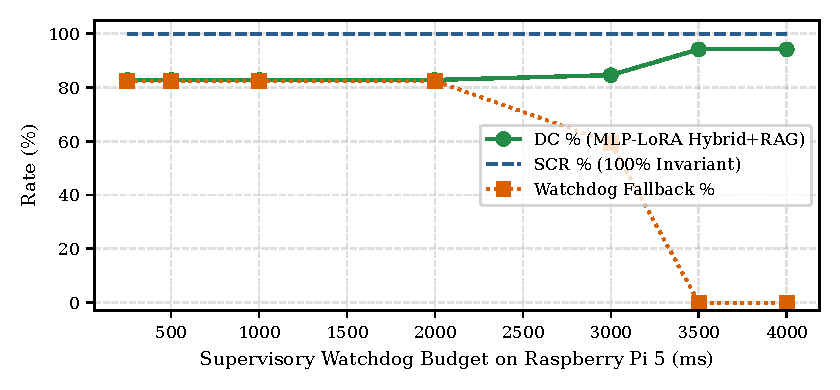
\includegraphics[width=0.48\textwidth]{figures/fig3_watchdog_tradeoff_pi5.pdf}
\caption{Supervisory watchdog budget trade-offs on Raspberry Pi 5 comparing fallback frequency, decision concordance, and safety invariance.}
\label{fig:watchdog}
\end{figure}

\subsection{Determinism and Real-Time Latency of the ANSI C Shield}
Table~\ref{tab:c_shield_rt} and Fig.~\ref{fig:rt} document the execution jitter of $\TotalCShieldCycles$ evaluations of the MONA-compiled ANSI C shield across standard and $\textsc{Preempt\_RT}$ kernels with core isolation ($\text{isolcpus}=3$).

\begin{table}[t]
\centering
\caption{MONA-Compiled ANSI C Shield Execution Latency on Raspberry Pi 5 ($10^7$ Cycles per Regime)}
\label{tab:c_shield_rt}
\begin{tabular}{lccccc}
\toprule
\textbf{Kernel / Scheduling Regime} & \textbf{$\mu$ (ns)} & \textbf{p50} & \textbf{p99} & \textbf{p99.99} & \textbf{Max ($\mu$s)} \\
\midrule
Standard Kernel (SCHED\_OTHER, Idle) & 56.46 & 56 & 75 & 93 & 48.33 \\
Standard Kernel (SCHED\_FIFO 80, Idle) & 56.20 & 56 & 75 & 93 & 13.72 \\
Standard Kernel (SCHED\_FIFO 80 + Load) & 56.09 & 56 & 75 & 93 & 18.63 \\
PREEMPT\_RT + isolcpus=3 (Idle) & 56.19 & 56 & 75 & 93 & 15.37 \\
PREEMPT\_RT + isolcpus=3 (+ Load) & 56.21 & 56 & 75 & 93 & 9.31 \\
\bottomrule
\end{tabular}
\end{table}


\begin{figure}[t]
\centering
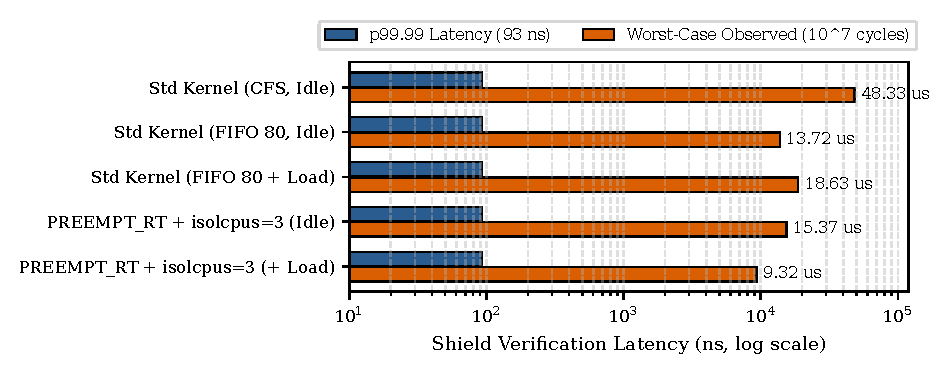
\includegraphics[width=0.48\textwidth]{figures/fig4_c_shield_rt_tail.pdf}
\caption{Tail latency distribution ($p99.99$ vs. worst-case observed) of the MONA-compiled ANSI C runtime guard across scheduling regimes.}
\label{fig:rt}
\end{figure}

\end{sec}

\begin{sec}{IV. CONCLUSION}
The MCAF architecture successfully reconciles neuro-symbolic SLM autonomy with hard real-time safety in autonomous mining systems. Future work will extend MCAF to multi-agent decentralized coordination fleets under adversarial wireless constraints.
\end{sec}

\begin{thebibliography}{1}
\bibitem{ref1} B. H. N. Andrade and R. A. R. Oliveira, ``Towards Resilient Agentic Mining: An Architectural Framework using Model Context Protocol and Deterministic Safety Guardrails,'' in \emph{Proc. ICEIS AXPRO}, 2026.
\end{thebibliography}

\end{document}
